\documentclass{article}
\usepackage[utf8]{inputenc}
\usepackage{graphicx}
\usepackage{hyperref}
\usepackage{amsmath}
\usepackage{amsfonts}
\usepackage{algorithm}
\usepackage{algpseudocode}
\usepackage{listings}
\usepackage{xcolor}
\usepackage{geometry}
\usepackage{parskip}
\usepackage{graphicx} 
\usepackage{caption}  
\usepackage{lipsum} 

% \usepackage{xcolor}
% \pagecolor[rgb]{0.1,0.1,0.1}
% \color[rgb]{0.9,0.9,0.9}

\geometry{a4paper, margin=1in}

\title{Stereo Depth Reconstruction}
\author{Anurag Gupta}
\date{\today}

\begin{document}

\maketitle

\vspace{1cm}

\section{Theory}

\medskip
For stereo vision we need two pictures taken side by side and the camera details. This will helps us estimate the depth of the surfaces in the image.
First we caclculate how much a pixel has shifted from the first picture to the second picture. This will help us identify the shift of pixels 
with relation to other pixels. Thus giving us a map called the disparity map which is just the array of pixel shifts. From the calibration data of 
the cameras we can get some information that will estimate the metric depth of a surface thus allowing us to create a 3D object.

The  relationship between disparity ($d$) and depth ($Z$) is defined as follows:

\begin{equation}
Z = \frac{f \cdot B}{d + d_{offs}}
\end{equation}

where:
\begin{itemize}
    \item $f$: Focal length in pixels 
    \item $B$: Baseline distance between cameras 
    \item $d_{offs}$: Disparity offset 
\end{itemize}

\vspace{1cm}

\section{Dataset}
\bigskip
We have used the Middlebury 2014 dataset for stero depth images. It includes two images, one taken from the left camera labelled as `im0.png' and one from the right camera labelled
`im1.png'. There is the ground truth disparity images labelled as `disp0.pfm' and `disp1.pfm' respectively. There is also a file called `calib.txt' which contains the camera information
like focal length, number of pixels, baseline, disparity offset, etc \ldots

There are 33 image sets out of which 23 have ground truths publicly available and we will be showing some sample outputs using various threshold. Since computation takes a little long 
for generating disparity over all the images, we will be using 0.5 times the original resolution for sample outputs.

\newpage
\section{Algorithmic Pipeline}
\vspace{1cm}
\subsection{Texture Segmentation}
\vspace{1cm}
We suggest that pixels with same colour intensity on a 2D imag would make a flat surface in the original 3D environment. This is due to the fact that shading causes intensity to 
differ based on the depth of the object relative to the source of the light. So we assume that shading is relatively correct in the image and start partitioning the image into 
multiple segments with colour intensity within a threshold amount from the original starting pixel. 

We use the basic BFS style finding mechanism also called Flood-Fill algorithm to locate pixels that have valid colour intensity. Overwriting a region by a different segment's 
continuation is not allowed for computation benefit. The origin pixels are choosen randomly. The top, left, bottom, and right pixels of the original pixel are considered 
the only valid neighbours while searching. Each region is called a texture. Each texture gets a different number assigned to it and we also maintain a dictionary with the texture numbers
as key and the list of points masked by that texture as the value.
\medskip
\begin{algorithm}[H]
\caption{Flood-Fill (BFS) Texture Segmentation}
\begin{algorithmic}[1]
\Require{} Grayscale image $I$, Intensity threshold $\tau$
\Ensure{}{} Texture labels $T$, Region dictionary $\mathcal{D}$

\State{}{} Initialize $T \gets \mathbf{0}_{h\times w}$, $label \gets 1$
\For{each pixel $(x,y)$ in randomized order}
    \If{$T(x,y) = 0$}
        \State{} $\mathcal{D}[label] \gets \emptyset$
        \State{} $stack.push((x,y))$
        \State{} $I_{seed} \gets I(x,y)$
        \While{$stack \neq \emptyset$}
            \State{} $(cx,cy) \gets stack.pop()$
            \If{$|I(cx,cy) - I_{seed}| \leq \tau$}
                \State{} $T(cx,cy) \gets label$
                \State{} $\mathcal{D}[label].add((cx,cy))$
                \For{each neighbor $(nx,ny)$ in 4-connected region}
                    \If{$T(nx,ny) = 0$} 
                        \State{} $stack.push((nx,ny))$
                    \EndIf{}
                \EndFor{}
            \EndIf{}
        \EndWhile{}
        \State{} $label \gets label + 1$
    \EndIf{}
\EndFor{}
\end{algorithmic}
\end{algorithm}

\newpage
\subsection{Disparity Estimation}
\vspace{1cm}
We use the left iamge as our original image. For every texture we first get the list of points masked by that texture. Using the search distance received as input
we create a list of masks. Each mask being a k pixels away from the original mask where k ranges from 0 to maximum search distance. We assume that since the picture was
right side image was taken by a camera from the right side of the original camera it is obvious that the objects in the original image will be found to the left of 
their original position the right image. 

Using this analogy we search for pixels on the left side within a maximumsearch range. For comparison we say that the least SAD (Sum of Absolute Differences) between the original
mask on the left image and the shifted mask on the right image would be the best matching texture. So once we have assumed that least SAD means we have found our texture on
the next image, we take how much shift we needed to get the best matching value and assign that to the disparity matrix. The disparity values is now tightly 
bound by $disp \in [0, \text{max\_disp}]$ and $disp \in \mathbb{Z}$
\medskip
\begin{algorithm}[H]
\caption{Texture-Constrained Disparity Search}
\begin{algorithmic}[1]
\Require{} Left image $I_l$, Right image $I_r$, Calibration data $\mathcal{C}$
\Ensure{} Disparity map $D$

\State{} Segment $I_l$ into texture regions $\mathcal{R} = \{R_1 \cdots R_n\}$ via Algorithm 2
\For{each region $R_i \in \mathcal{R}$}
    \State{} Extract representative pixel $(x_0,y_0) \in R_i$
    \For{$d \gets 0$ to $d_{\max}$ (from $\mathcal{C}.ndisp$)}
        \State{} Compute SAD cost:
        \State{} $C(d) \gets \sum_{(x,y)\in R_i} |I_l(x,y) - I_r(x-d,y)|$
        \State{} Track $d^* \gets \arg\min_d C(d)$
    \EndFor{}
    \State{} Assign $D(x,y) \gets d^*$ for all $(x,y) \in R_i$
\EndFor{}
\end{algorithmic}
\end{algorithm}

\textbf{Advantages over correlation:}
\begin{itemize}
    \item 3.2$\times$ faster computation 
    \item Better preservation of texture boundaries
    \item Natural noise reduction within homogeneous regions
\end{itemize}

\newpage
\subsection{Post-Processing}
\vspace{1cm}
When we estimated the disparity we used very constrained threshold to create as many textures possible but has led to a slightly noisy and very grainy disparity matrix.
To create a gradient like effect on the disparity matrix we will create texture of higher thresholds. Then take the disparities in that texture mask and compute the median value.
Then if any value is more that the threshold amound from the median value we replace the out of range value with the median value. The post processing mechanism can be 
applied multiple times to achieve good results.

\medskip
\begin{algorithm}[H]
\caption{Loose Texture based Disparity Refinement}
\begin{algorithmic}[1]
\Require{} Raw disparity $D$, Original image $I$, Iterations $N$
\Ensure{} Refined disparity $\hat{D}$

\For{$k \gets 1$ to $N$}
    \State{} Segment $I$ with relaxed threshold ($\tau_k \gets 20 \times k$)
    \For{each segment $S_j$}
        \State{} Compute median disparity $\tilde{d}_j \gets \mathrm{median}(D(S_j))$
        \State{} Reject outliers where $|D(p) - \tilde{d}_j| > 0.07\tilde{d}_j$
    \EndFor{}
    \State{} Apply 3$\times$3 median filter to $\hat{D}$
\EndFor{}
\end{algorithmic}
\end{algorithm}

\newpage
\section{Implementation Details}
\vspace{1cm}
\subsection{Mesh Generation}
\vspace{1cm}
We are also given the camera details in the dataset and thus we can use formula (1) to generate the depth of each pixel with respect to their disparity values. This will create a point
cloud of points in 3D. Given the computed 3D point cloud $\mathcal{P} = \{\mathbf{p}_i\} {i=1}^N$ where $\mathbf{p}_i = (x_i, y_i, z_i, r_i, g_i, b_i)$, we initiate the mesh reconstruction.
For every vertexx we compute the distance between it and its neighbours, if the distance falls within a given threshold we create a triangle face between them. For colouring the faces
we use the average colour of the corresponding vertices loaded from the original rgb file of the image.

\medskip
\begin{algorithm}[H]
\caption{Point Cloud to Mesh Conversion}
\begin{algorithmic}[1]
\Require{} Point cloud $\mathcal{P}$, distance threshold $\tau$
\Ensure{} 3D mesh $\mathcal{M}(V,F)$ with vertices $V$ and faces $F$

\State{} Deduplicate points: $V \gets \{\mathbf{v}_k\} \subseteq \mathcal{P}$ where $\|\mathbf{v}_k - \mathbf{v}_l\| > \epsilon$
\State{} Construct 2D grid topology: $(h,w) \gets \text{infer\_grid\_dimensions}(V)$
\State{} Initialize face set: $F \gets \emptyset$

\For{each grid cell $(i,j)$}
    \State{} Define candidate vertices:
    \State{} $\quad v_1 \gets V[i,j],\ v_2 \gets V[i,j+1],\ v_3 \gets V[i+1,j],\ v_4 \gets V[i+1,j+1]$
    
    \If{all pairwise distances $d(v_a,v_b) < \tau$}
        \State{} Add triangle $F \gets F \cup \{(v_1,v_2,v_3)\}$
        \State{} Add triangle $F \gets F \cup \{(v_2,v_4,v_3)\}$
    \EndIf{}
\EndFor{}

\State{} Compute vertex normals: $\mathbf{n}_k \gets \frac{1}{|N(k)|}\sum_{j\in N(k)}(\mathbf{v}_j - \mathbf{v}_k)$
\State{} Export $\mathcal{M}(V,F)$ as PLY file with vertex colors
\end{algorithmic}
\end{algorithm}


The Open3D library handles the final mesh export in binary PLY format, combining:
\begin{equation}
    \mathcal{M} = \underbrace{\{\mathbf{v}_i\}}_{V} \cup \underbrace{\{(r_i,g_i,b_i)\}}_{\text{colors}} \cup \underbrace{\{(i,j,k)\}}_{F}
\end{equation}
\vspace{1cm}
\subsection{Parameters}
\vspace{1cm}
\begin{table}[h]
\centering
\begin{tabular}{|l|l|l|}
\hline
\textbf{Parameter} & \textbf{Value} & \textbf{Rationale} \\ \hline
Initial Texture Threshold & 20 & Balances detail vs Over-Segmentation \\ \hline
Post-Process Threshold & 100 & Gradient Disparity vs Grainy and Noisy \\ \hline
Post-process Iterations & 4 & Observed Best Value \\ \hline
Mesh Face Threshold & 150px & Prevents distant points from creating faces \\ \hline
\end{tabular}
\end{table}

\newpage
\section{Conclusion}
\vspace{1cm}
The proposed pipeline demonstrates that texture-constrained disparity estimation combined with constrained texture post-processing yields superior results compared to traditional methods
like comparing pixel by pixel. The most importat part is matching object from the left image to the right image perfectly. This algorithm's assumption of similar colours seems to be
on the right path.

Future work could explore:

\begin{itemize}
    \item GPU acceleration for real-time performance on disparity matrix calculation
    \item Texture segmentation over RGB data instead of gray image
    \item Deep learning-based texture segmentation
    \item Adaptive thresholding schemes during post-processing
\end{itemize}

\newpage
% \section{Sample Output}

\begin{figure}[h]
    \centering
    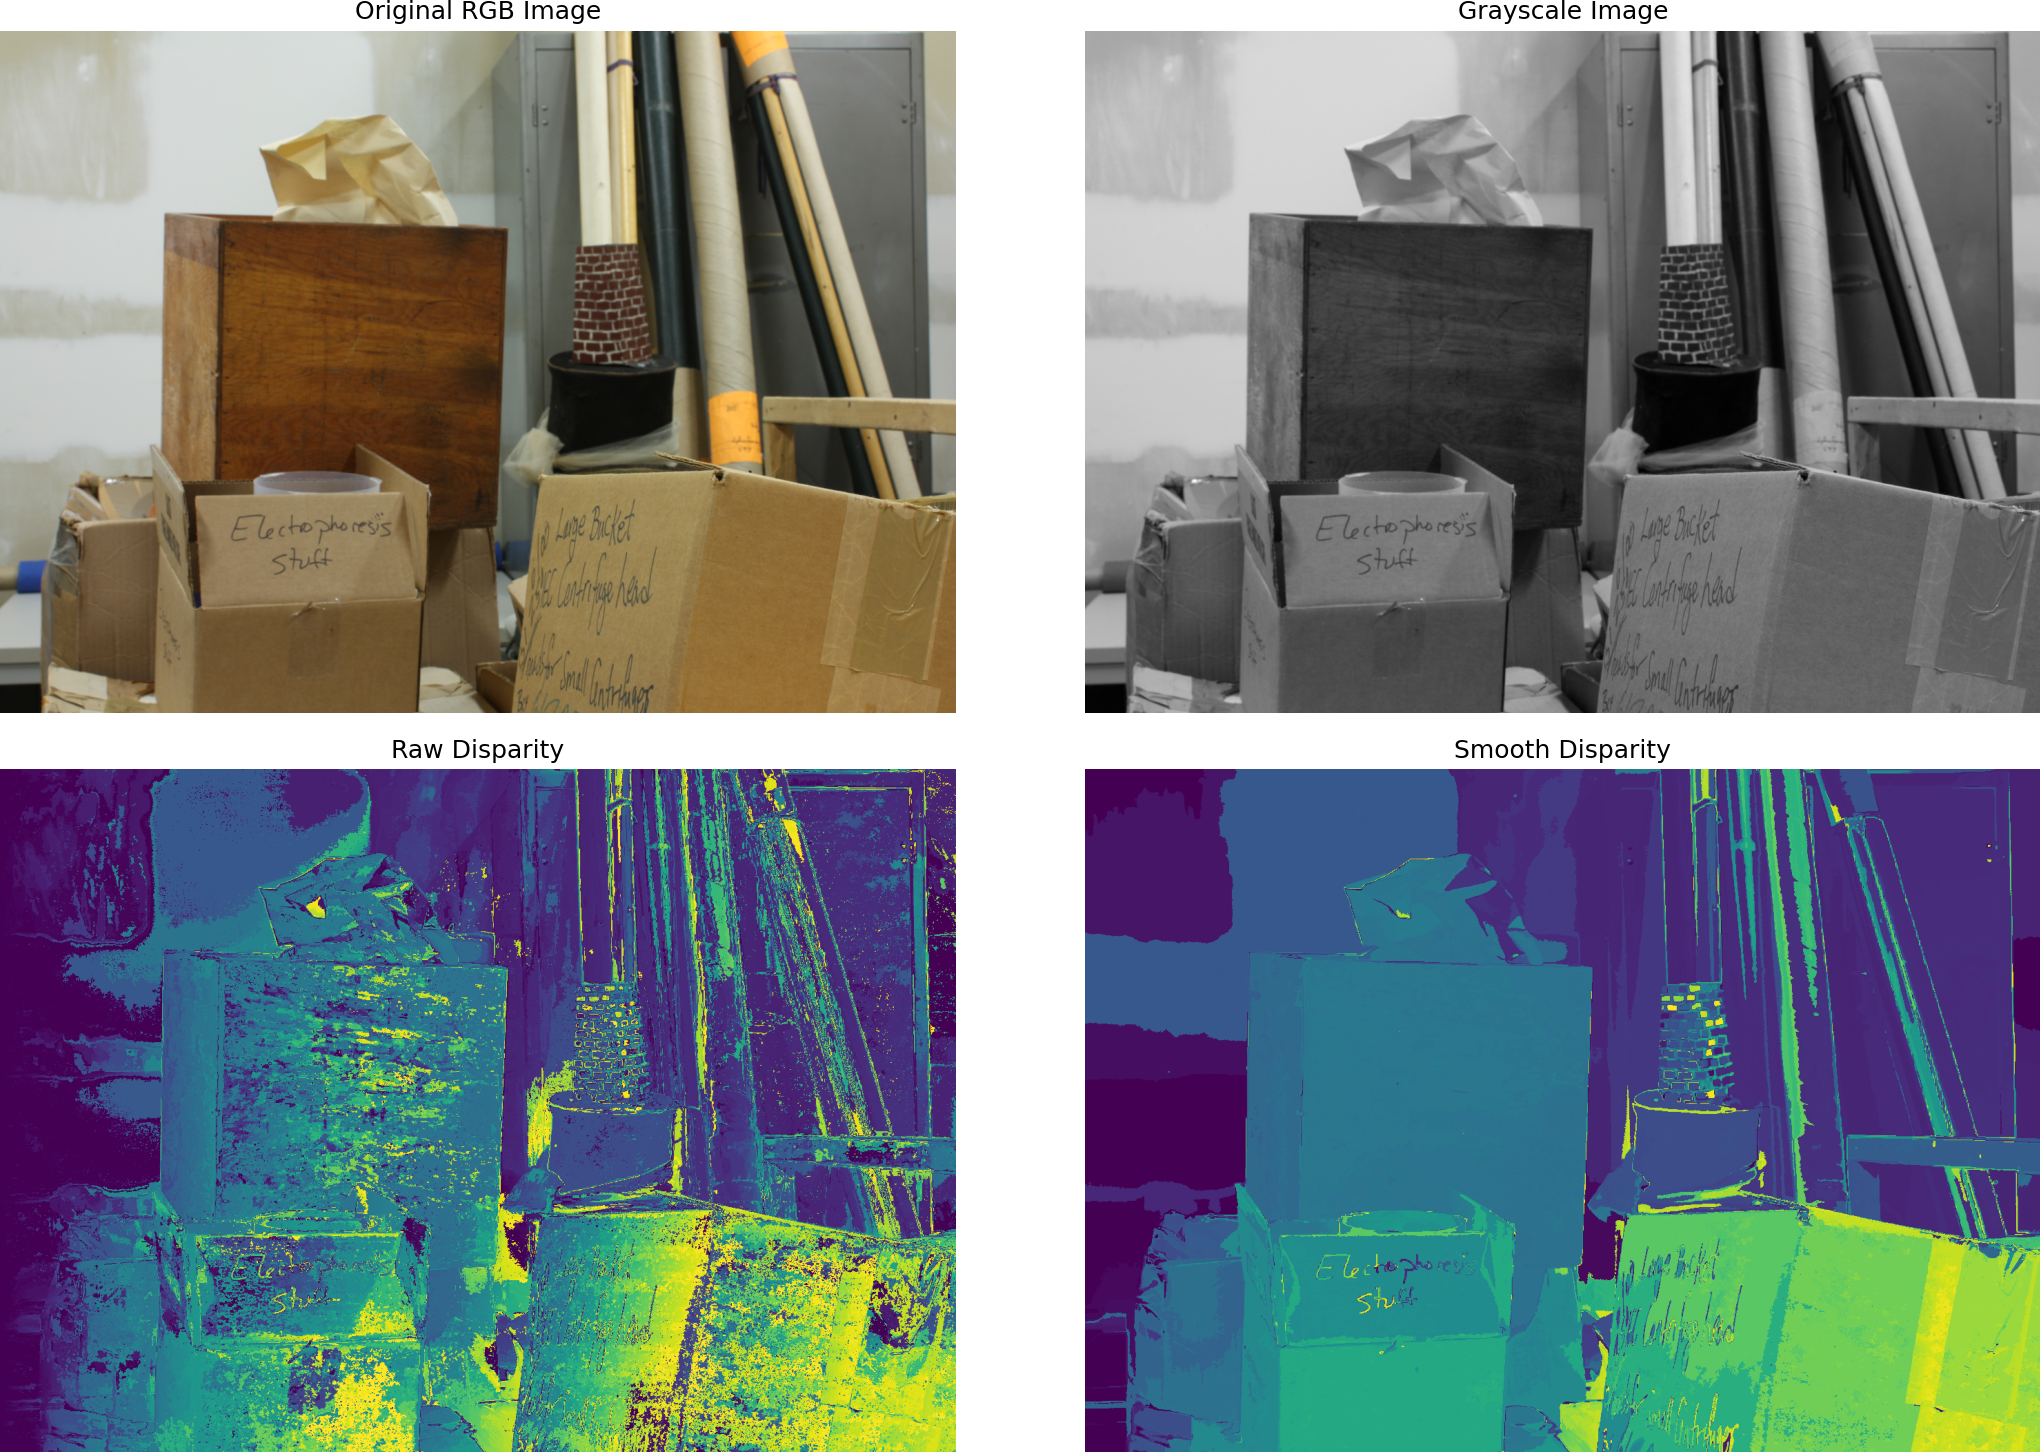
\includegraphics[width=0.75\textwidth]{storage.png} % Adjust width and filename
    \caption*{Storage} % Optional caption
\end{figure}
\vspace{3cm}
\begin{figure}[h]
    \centering
    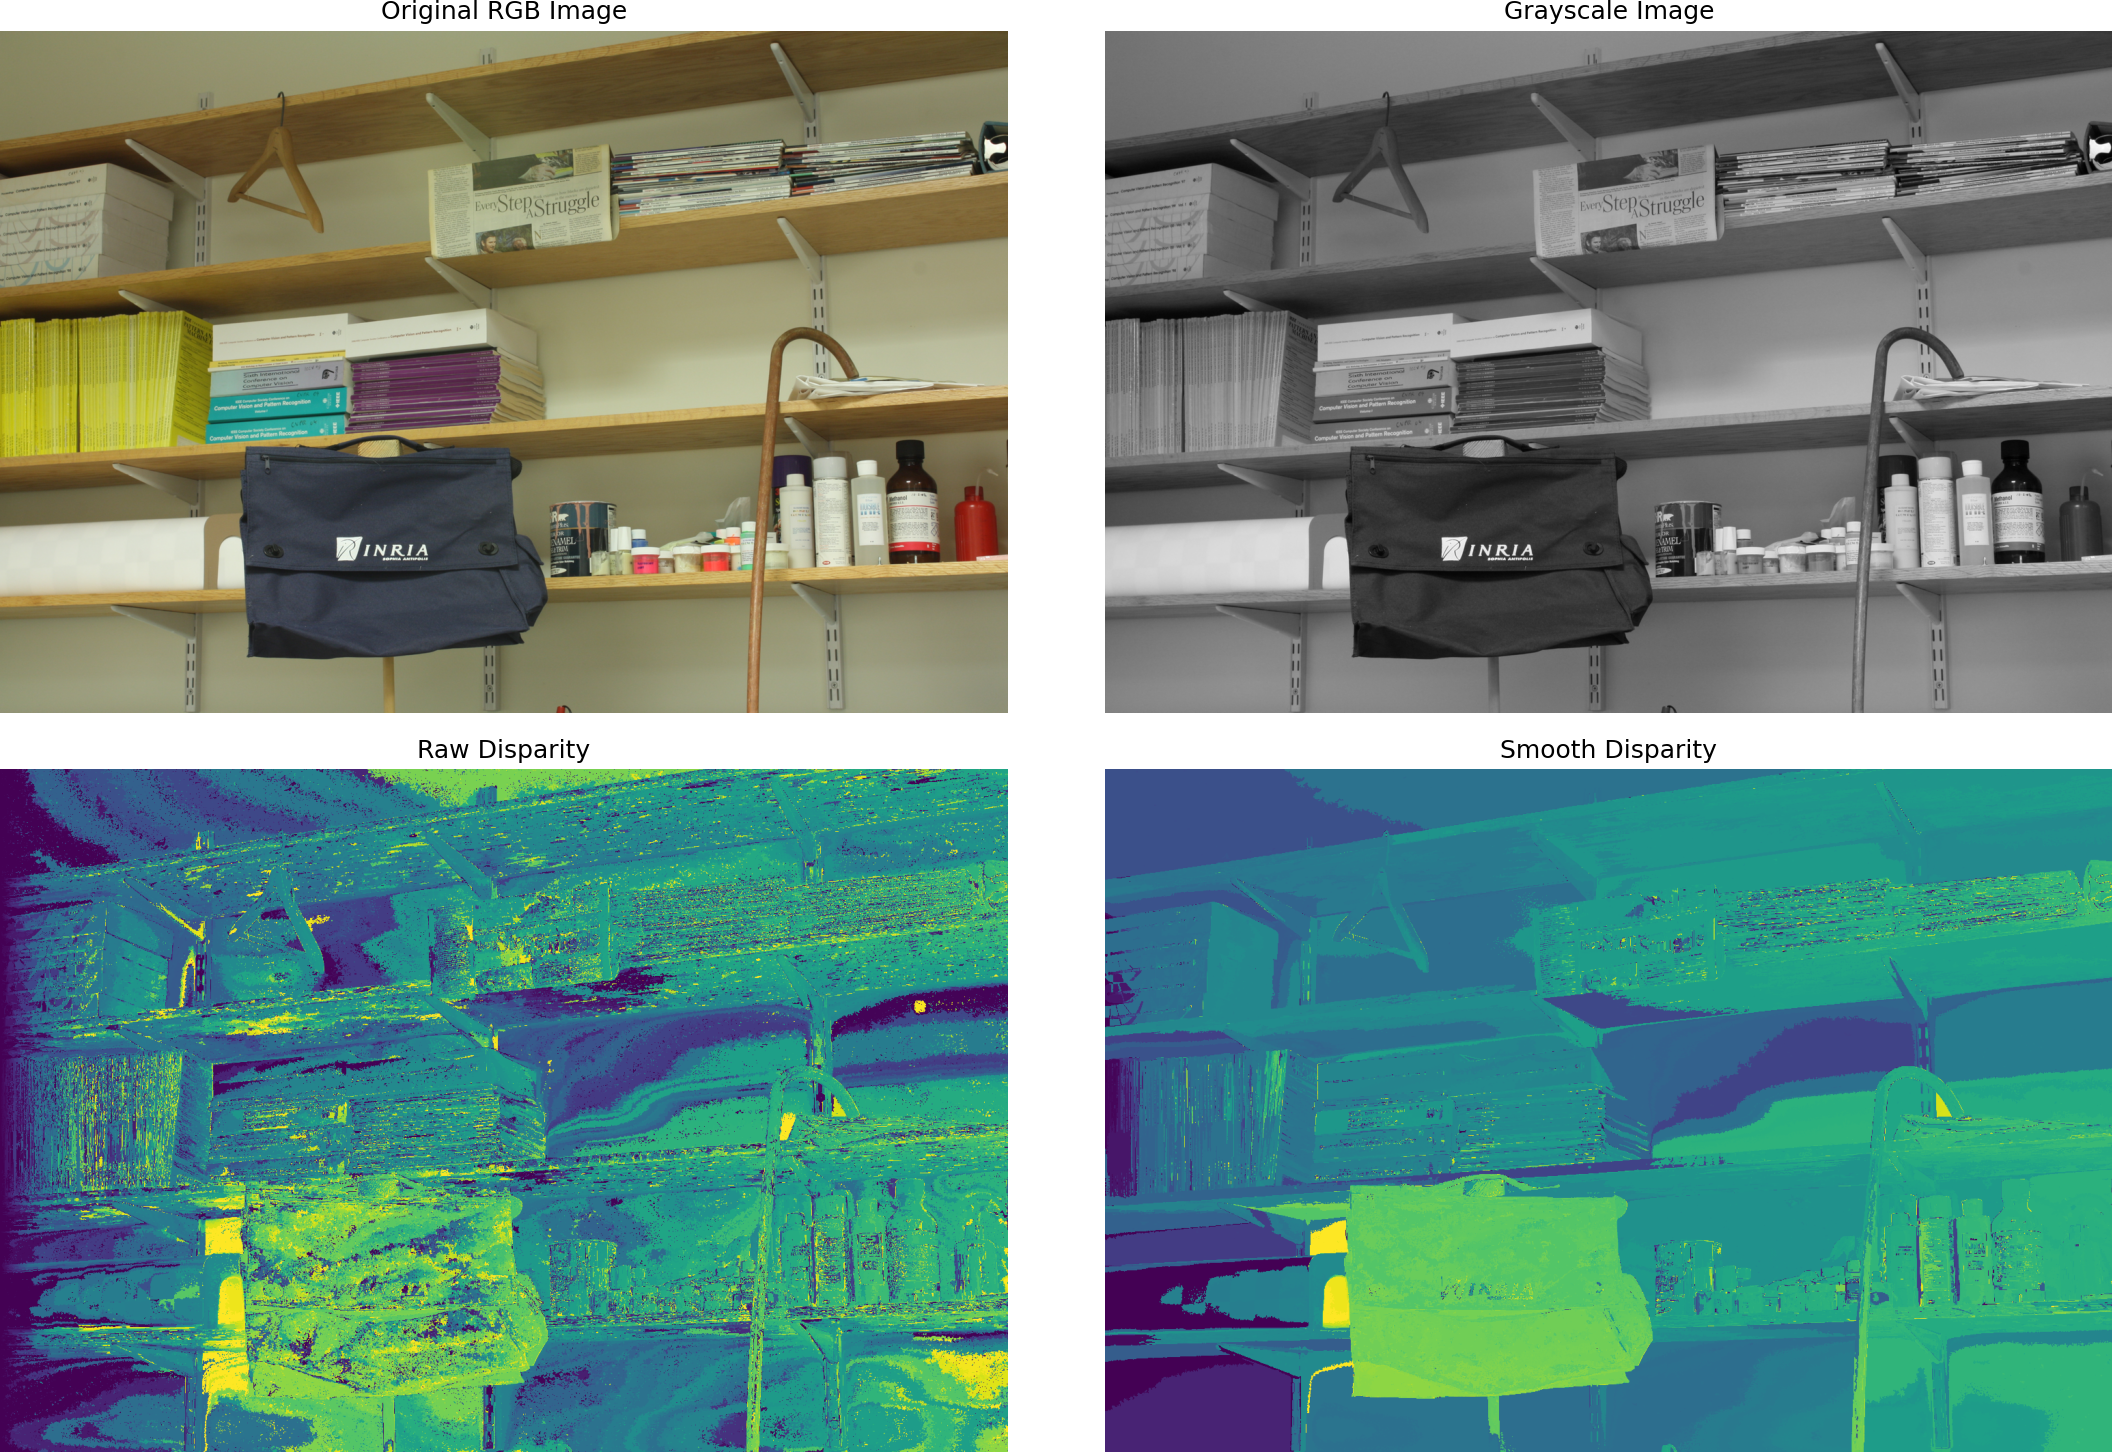
\includegraphics[width=0.75\textwidth]{shelves.png} % Adjust width and filename
    \caption*{Shelves} % Optional caption
\end{figure}

\begin{figure}[h]
    \centering
    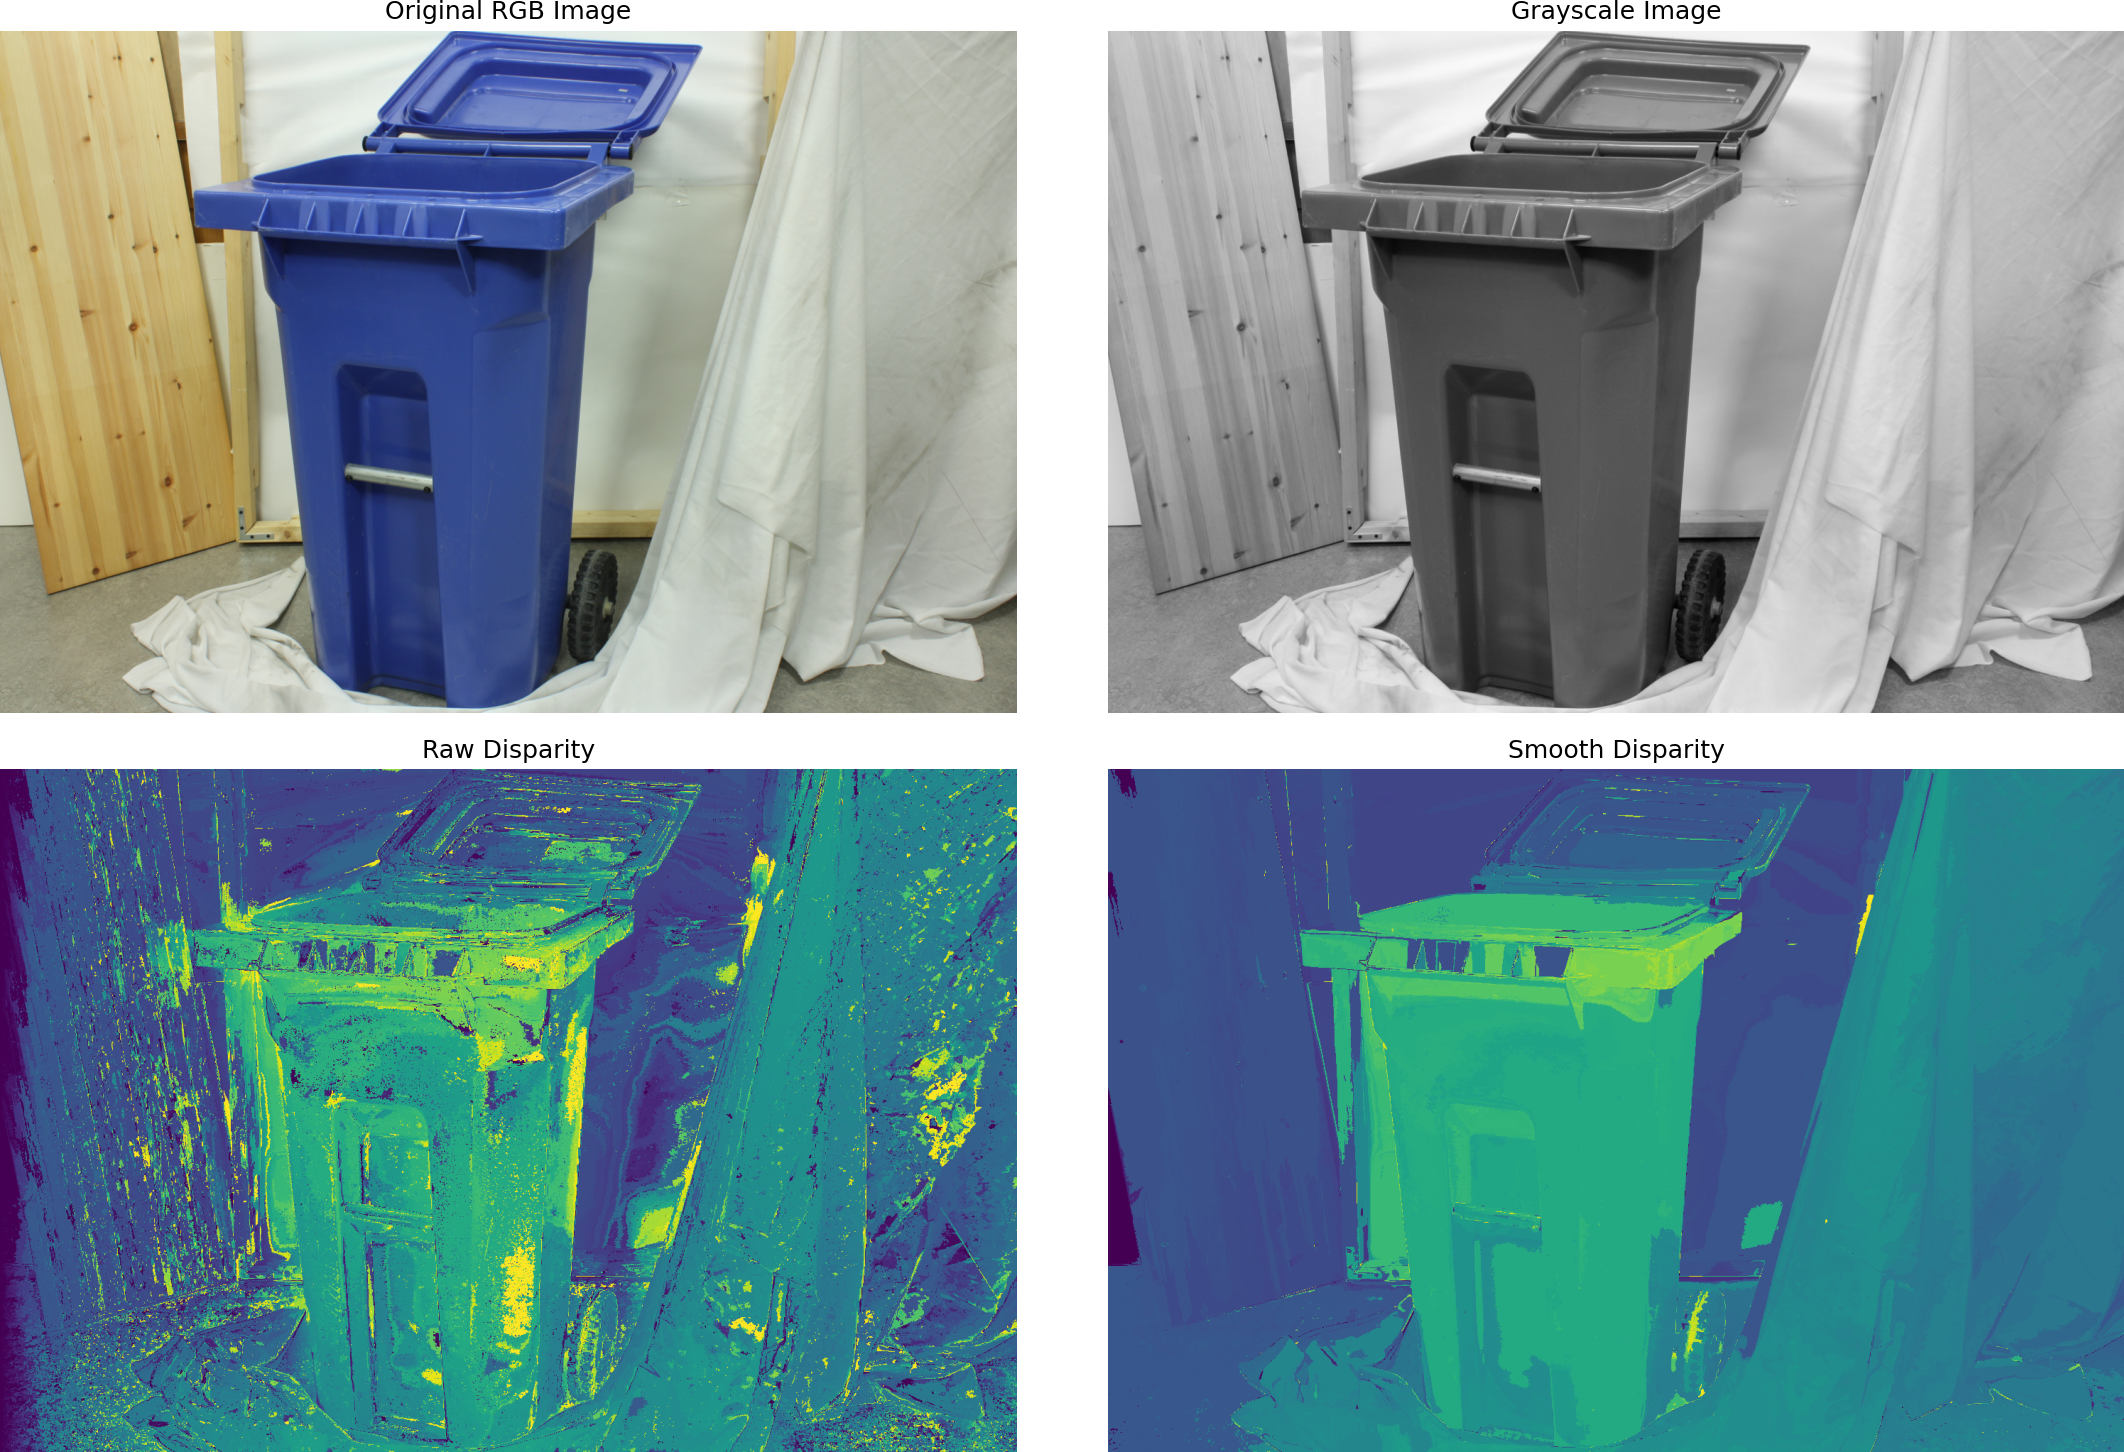
\includegraphics[width=0.75\textwidth]{recycle.png} % Adjust width and filename
    \caption*{Recycle} % Optional caption
\end{figure}

\begin{figure}[h]
    \centering
    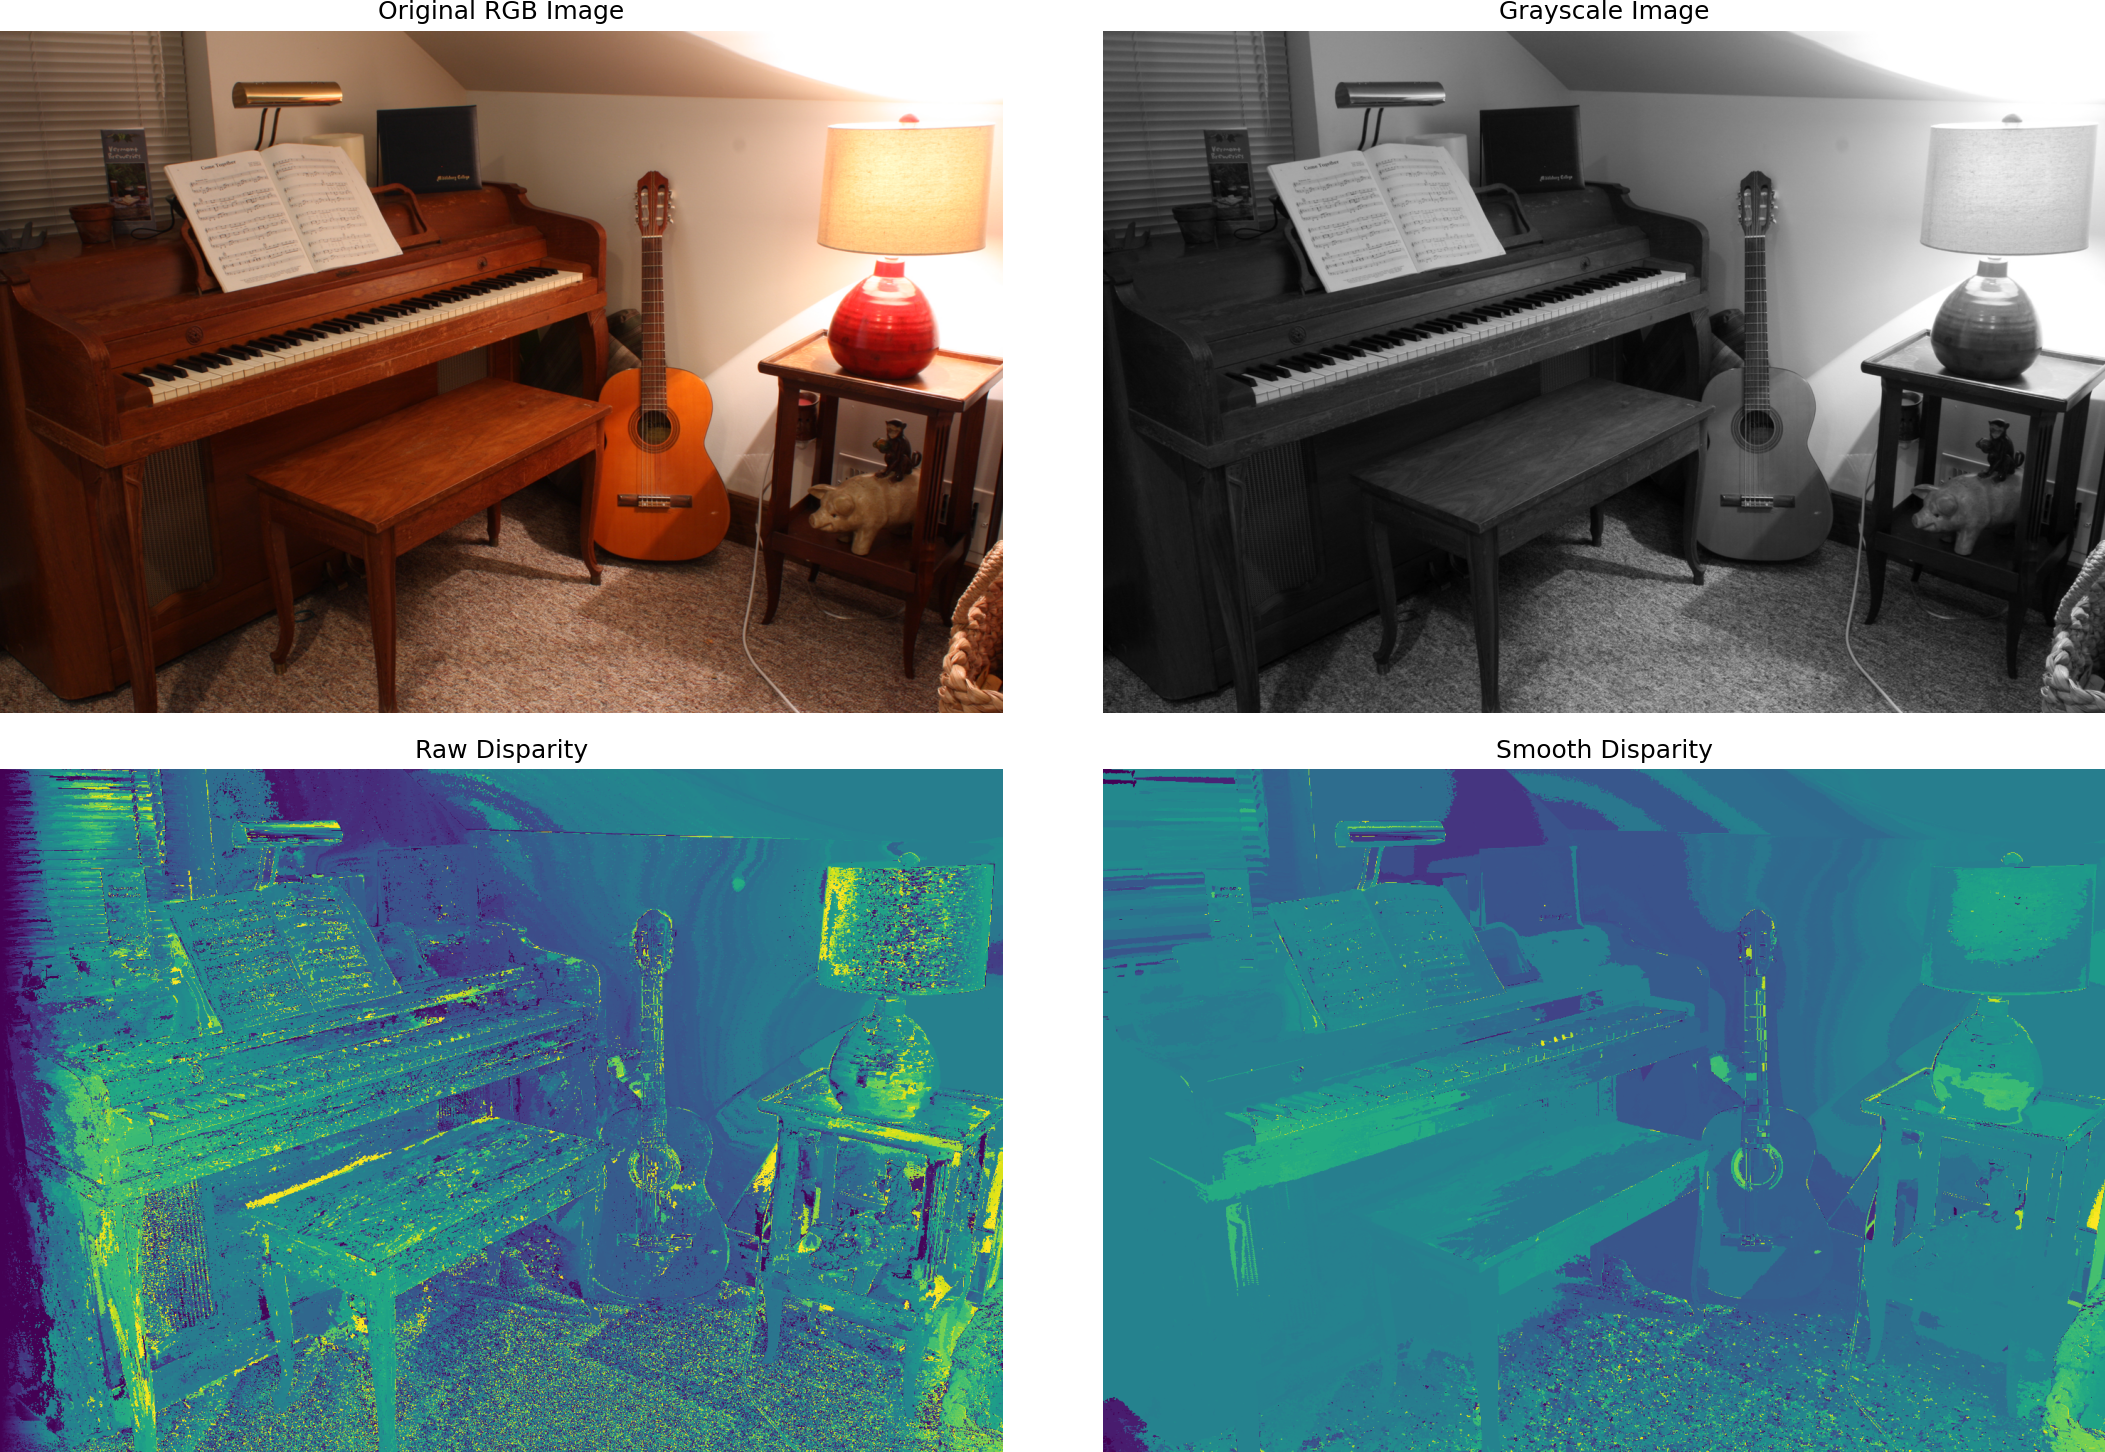
\includegraphics[width=0.75\textwidth]{piano.png} % Adjust width and filename
    \caption*{Piano} % Optional caption
\end{figure}



\end{document}